% !TEX encoding = UTF-8 Unicode
\documentclass[a4paper,9pt]{article} 
\usepackage[utf8]{inputenc}
\usepackage{enumerate} %for roman numbers, letters ect.
\usepackage{listings}
\usepackage{amsmath}
\usepackage{amsfonts}
\usepackage{amssymb}
\usepackage{placeins}
\usepackage{algorithmicx}
\usepackage{csquotes}
\usepackage{graphicx}
\usepackage{hyperref}
\usepackage[colorlinks]{hyperref}
\graphicspath{ {figures/} } 

\newcommand{\NBvK}{\mathcal{N}_\text{BvK}}
\newcommand{\LBvK}{\mathcal{L}_\text{BvK}}

\begin{document}
%	\centering
\begin{centering}
	{\scshape\Large  Signifikans, statistikk og eksperimentelle data. \par}
	\vspace{1cm}
	{\scshape\Large Tips og triks    \par}
	\vspace{1.5cm}
	{\huge\bfseries \par}
	\vspace{2cm}
	%{\Large\itshape  \par}

 %Bottom of the page
	{\large \today\par}
\end{centering}


\tableofcontents

\pagebreak

\section{Kort om teksten}

Dette dokumentet er ment å gi en kortfattet og superenkel guide til bruk av:

\begin{itemize}
\item Signifikans (\emph{antall signifikante siffer, antall desimaler, regneoperasjoner med korrekt antall signifikante siffer og desimaler}).
\item Eksperimentelle data (\emph{resultater fra laboratorieforsøk, undersøkelser eller observasjoner}).
\item Statistikk (\emph{matematiske regler for å behandle, tolke og presentere data}).
\end{itemize}

Hensikten er at du på noen timer skal kunne lære deg alt du trenger for å mestre disse verktøyene.  Det krever selvfølgelig litt innsats fra din side også. Hver seksjon er på noen få linjer, og jeg har forsøkt så godt som mulig å sikre at disse få linjene inneholder alt du trenger å vite om saken (for nå, i det minste). Det som er din oppgave er å \emph{forstå} hva som står der. Det innebærer å \emph{lese} teksten, men også å \emph{tenke} over det du leser. Om noe virker uklart, rart eller uforståelig kan du lene deg tilbake, se litt opp i taket og tenke nøye gjennom over hva du nettopp har lest. Kanskje klarner det, kanskje ikke. I verste fall er det jeg som har skrevet noe feil, og i så fall håper jeg du kan sende meg en e-post på \href{mailto:audunsh4@gmail.com}{audunsh4@gmail.com}, så skal jeg fikse det så fort som mulig.

\vspace{.5cm}

Å studere vitenskap er litt som å drive med mental kampsport. Jeg er helt sikker på at du vil få dette til, men ta i mot et råd fra en 900 år gammel Jedi-mester: \emph{"Do, or do not. There is no try."}. Lykke til! :)

\vspace{.5cm}

\begin{flushright}
Med vennlig hilsen Audun
\end{flushright}


\pagebreak

\section{Oversikt}

Her er en oversikt over hva du bør kunne etter å ha lest dokumentet:

\begin{itemize}
\item Signifikans. Du bør kunne
\begin{itemize}
\item Telle antall signifikante siffer og antall desimaler.
\item Utføre aritmetiske operasjoner som multiplikasjon, divisjon, addisjon og subtraksjon med riktig antall gjeldende siffer og desimaler.
\end{itemize}
\item Statistikk. Du bør
\begin{itemize}
\item Kunne beregne gjennomsnitt, standardavvik og standardfeil.
\item Kjenne til begrepet \emph{populasjonens gjennomsnitt} og kunne skille mellom dette og \emph{utvalgets gjennomsnitt}.
\item Kjenne til forskjellen mellom standardfeil og standardavvik, og kunne redegjøre for når det er hensiktsmessig å bruke det ene eller andre.
\end{itemize}
\item Behandling av eksperimentelle data. Du bør
\begin{itemize}
\item Kunne benytte reglene for signifikans for å unngå falsk presisjon i gjengivelse av eksperimentelle data.
\item Kunne redegjøre for sammenhengen mellom standardavvik, standardfeil og måleusikkerhet.
\item Kunne redegjøre for begrepene presisjon og nøyaktighet, og relatere disse til statistiske størrelser.
\item Kjenne til enkel feilforplantning.
\item Kjenne til noen vanlige konvensjoner for gjengivelse av eksperimentelle data.
\end{itemize}
\end{itemize}


%Bias/unbiased (n, n-1)



%I dette dokumentet finner du en oversikt 

%Dette dokumentet gir en oversikt over regler og konvensjoner som det forventes at studentene i KJM1101 skal  beherske.

%Vi ser først på regnereglene isolert, deretter relaterer vi disse til behandling av eksperimentelle data og statistisk analyse. 

\pagebreak

\section{Desimaler og signifikante siffer}

\framebox[1.1\width]{\href{https://www.khanacademy.org/math/arithmetic-home/arith-review-decimals/arithmetic-significant-figures-tutorial/v/significant-figures}{Læringsressurs: Kahn Academy - Significant Figures (video, lenke)}}

\vspace{.5cm}

Du bør kunne

\begin{itemize}
\item Telle antall signifikante siffer og antall desimaler.
\item Utføre aritmetiske operasjoner som multiplikasjon, divisjon, addisjon og subtraksjon med riktig antall gjeldende siffer og desimaler.
\end{itemize}

For å få til dette må du først lære deg å telle desimaler og signifikante siffer, og deretter lære deg de to enkle reglene for aritmetiske operasjoner på tallene.

\subsection{Antall desimaler}

Du finner antallet desimaler i et tall ved å \textbf{telle alle siffer etter komma}. Her er noen eksempler:

\begin{itemize}
\item $1$ har ingen desimaler.
\item $1.\mathbf{0}$ har 1 desimal. 
\item $1.\mathbf{0000}$ har 4 desimaler. 
\end{itemize}

\subsection{Summasjon av reelle tall}

Når du \textbf{summerer} reelle tall skal resultatet rundes av til like mange desimaler som\textbf{ leddet med færrest} desimaler. Her er noen eksempler:

\begin{itemize}
\item $1 + 1.0 = 2$.
\item $1.23 + (- 1.1) = 0.1$.
\item $1.000 + 1.0 = 2.0$. 
\end{itemize}



\subsection{Antall signifikante siffer}

Du finner antallet signifikante siffer ved å telle fra venstre mot høyre alle oppgitte siffer fra og med første siffer ulikt 0. Her er noen eksempler (pass på at du er enig i dem alle):

\begin{itemize}
\item $\mathbf{1}$ har 1 signifikant siffer.
\item $\mathbf{1.0}$ har 2 signifikante siffer. 
\item $0.\mathbf{12345}$ har 5 signifikante siffer. 
\item $0.000\mathbf{12345}$ har 5 signifikante siffer. 
\item $\mathbf{1.02}$ har 3 signifikante siffer. 
\item $\mathbf{2.0}\cdot10^{-2}$ har 2 signifikante siffer. 
\end{itemize}

Ikke bli forvirret av nullene. Alle de følgende måtene å skrive tallet $\mathbf{2.0000}\cdot10^{-2}$ på har 5 signifikante siffer:

\begin{equation}
\mathbf{2.0000}\cdot10^{-2} = 0.020000 = \mathbf{20000}\cdot10^{-6} 
\end{equation}

\subsection{Noen unntak ved telling av signifikante siffer}

Det finnes noen få unntak når du teller signifikante siffer. Disse er:

\begin{itemize}
\item Enkelte størrelser, slik som heltall (1,2,3...) og noen konstanter ($\pi$, $e$), kan antas å ha uendelig mange signifikante siffer, slik at de ikke påvirker endelig resultat. Et eksempel er konverteringen fra Torr til atomsfære i lab 2. Et annet er når man beregner volum av en sylinder basert på måling av diameter og høyde.
\end{itemize}

\subsection{Multiplikasjon og divisjon med signifikante siffer}

Når du \textbf{multipliserer (eller dividerer)} reelle tall skal resultatet rundes av til samme antall signifikante siffer som \textbf{faktoren\footnote{eller dividend, divisor.} med færrest} signifikante siffer. Her er noen eksempler:

\begin{equation}
\frac{1.23}{2.0} = 1.23 \cdot 0.50 = 0.62 
\end{equation}

\begin{equation}
\frac{1.234}{2.0} = 0.62
\end{equation}

\begin{equation}
\frac{1.23}{2.00} = 0.615
\end{equation}

\begin{equation}
\frac{1.23}{2.000} = 0.615
\end{equation}

\pagebreak

\section{Statistikk}

\framebox[1.1\width]{\href{https://www.khanacademy.org/math/statistics-probability/sampling-distributions-library/sample-means/v/statistics-sample-vs-population-mean}{Læringsressurs: Kahn Academy - Sampling distribution of a sample mean (video, lenke)}}

\vspace{.5cm}

Etter å ha gjennomgått denne seksjonen bør du:

\begin{itemize}
\item Kunne beregne gjennomsnitt, standardavvik og standardfeil.
\item Kjenne til begrepet \emph{populasjonens gjennomsnitt} og kunne skille mellom dette og \emph{utvalgets gjennomsnitt}.
\item Kjenne til forskjellen mellom standardfeil og standardavvik, og kunne redegjøre for når det er hensiktsmessig å bruke det ene eller andre.
\end{itemize}

\subsection{Noen begreper}

En \emph{populasjon} er for vårt anliggende gitt ved alle mulige utfall av en måling. Som regel kan vi ikke gjøre alle mulige målinger, men må heller ta til takke med et begrenset antall målinger som vi antar er representative for populasjonen. En slik begrenset mengde målepunkter kalles et \emph{utvalg}. 
Fra et slikt utvalg kan vi beregne en rekke størrelser\footnote{I statistikk kalles disse størrelsene for "statistics", for å skille de fra "parameters" som er de tilsvarende størrelsene for populasjonen.} slik som \emph{gjennomsnitt}, \emph{standarfeil} og \emph{standardavvik}, og ønsker å benytte disse for å si noe om populasjonen som helhet.

\vspace{.5cm}

En kortfattet oppsummering av nye ord:
\begin{itemize}
\item \emph{Populasjon} - mengden av alle mulige målinger.
\item \emph{Utvalg} - en begrenset menge målinger tatt fra populasjonen.
\item \emph{Populasjonens gjennomsnitt} - Det "sanne" gjennomsnittet, beregnet fra alle mulige målinger.
\item \emph{Utvalgets gjennomsnitt} - Gjennomsnittet beregnet fra utvalget.
\item \emph{Parameter} - Størrelser beregnet fra populasjonen.
\item \emph{Statistic} - Størrelser beregnet fra utvalget.
\end{itemize}

\subsection{Gjennomsnitt}

Gjennomsnittet $\bar{x}$ i et utvalg $x_i$ er gitt ved

\begin{equation}
\label{eqn:mean}
\bar{x} = \frac{1}{N} \sum_{i=1}^N x_i = \frac{1}{N}(x_1 + x_2 + ... + x_N),
\end{equation}

hvor $N$ er antall målinger\footnote{samples}.

\vspace{.5cm}

Vi skiller mellom populasjonens gjennomsnitt og utvalgets gjennomsnitt, da det som regel er det siste vi måler. 

\begin{figure}[h]
\label{fig:standardfeil}
\centering
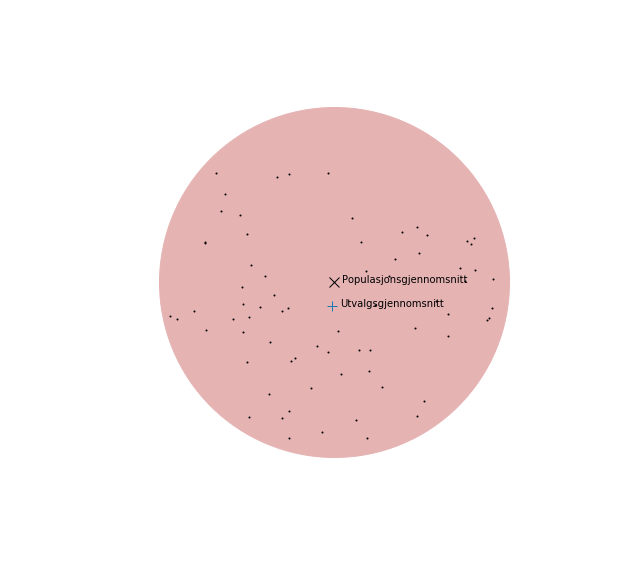
\includegraphics[width=\textwidth]{population}
\caption{Populasjon angitt med rødt, utvalget representert ved sorte punkter. Populasjonens gjennomsnitt $\bar{\mu}$ er gjennomsnittet av alle mulige målinger. Utvalgets gjennomsnitt $\bar{x}$ beregnes derimot fra et begrenset utvalg fra populasjonen. Vi antar at det er mulig å nærme seg  populasjonens gjennomsnitt ved å øke antallet målinger. Avstanden mellom $\bar{\mu}$ og $\bar{x}$ antas å være relatert til utvalgets standardfeil. Presisjonen i målingene relateres derimot ofte til målingenes standardavvik.}
\end{figure}

\subsection{Standardfeil}

Standardfeilen $SE$ regnes ut ved

\begin{equation}
\label{eqn:standarderror}
SE = \frac{1}{N} \sqrt{\sum_{i=1}^N (x_i - \bar{x})^2}.
\end{equation}

Det er mulig å vise\footnote{For en mer utfyllende forklaring se læringsressurs gitt innledningsvis i seksjonen.} at standardfeilen er relatert til standardavviket i utvalgets gjennomsnitt, med andre ord at avstanden mellom populasjonen og utvalgets gjennomsnitt er relatert til standardfeilen, som vist i figur 1. 

\FloatBarrier

\subsection{Standardavvik}

Standardavviket i et utvalg kan regnes ut fra standardfeilen ved

\begin{equation}
\label{eqn:standarddev}
\sigma = \sqrt{N} \cdot SE =\frac{1}{\sqrt{N}} \sqrt{ \sum_{i=1}^N (x_i - \bar{x})^2} .
\end{equation}

Hvor $N$ er antall målinger. Det er vanlig å regne ut standardavviket direkte fra det siste uttrykket over, og deretter standardfeilen ved å dele på $\sqrt{N}$.\footnote{Legg gjerne merke til at vi her har brukt faktoren $\frac{1}{\sqrt{N}}$. Dette er for å holde ligningene rene og pene. Når standardavviket defineres med faktoren $\frac{1}{\sqrt{N-1}}$  kalles det for "Bessel's korreksjon", og hensikten er å ikke underestimere standardavviket.}

\begin{figure}[h]
\centering
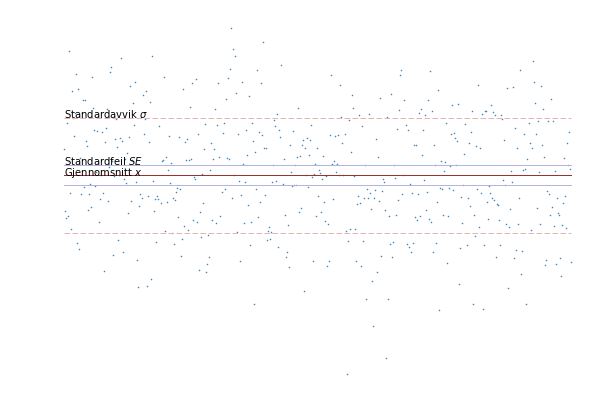
\includegraphics[width=\textwidth]{standardfeil1}
\caption{Standardavvik og standardfeil for et datasett.}
\end{figure}
 
\begin{figure}[h]
\centering
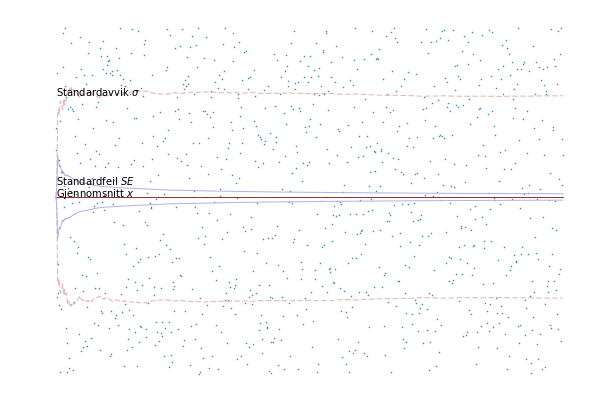
\includegraphics[width=\textwidth]{standard_n}
\caption{Standardavvik og standardfeil som funksjon av antall målinger (øker mot høyre).}
\end{figure}



 
\FloatBarrier

\pagebreak 
 
\section{Behandling av eksperimentelle data}

Etter å ha lest denne seksjonen bør du:
\begin{itemize}
\item Kjenne til enkel feilforplantning.
\item Kunne benytte reglene for signifikans for å unngå falsk presisjon i gjengivelse av eksperimentelle data.
\item Kunne redegjøre for sammenhengen mellom standardavvik, standardfeil og måleusikkerhet.
\item Kunne redegjøre for begrepene presisjon og nøyaktighet, og relatere disse til statistiske størrelser.
\item Kjenne til noen vanlige konvensjoner for gjengivelse av eksperimentelle data.
\end{itemize}

\subsection{Motivasjon: enkel feilforplantning}

De fleste eksperimentelle målinger vil ha en feilmargin, hvilket betyr at utfallet av målingen kan skrives på formen 

\begin{equation}
\label{eqn:precision}
x_0 \pm \Delta x.
\end{equation}

Her er $x_0$ den målte verdien og $\Delta x$ er oppgitt eller beregnet for måleinstrumentet som benyttes.  Når man gjør aritmetiske operasjoner på slike størrelser er det formelt korrekt å ta med feil-estimatet i operasjonene. Dette kalles for å la feilen "forplante seg" eller "propagere". For eksempel vil produktet av en måling og en eksakt kjent størrelse $a$ kunne skrives som

\begin{equation}
\label{eqn:propagation}
a(x_0 \pm \Delta x)=ax_0 \pm \vert a \vert \Delta x.
\end{equation}

Som det fremgår av uttrykket ovenfor blir feilen skalert mot størrelsen $a$. Om eksempelvis $a=10$ vil også feilen øke med en størrelsesorden. Om vi ikke hadde latt feilen forplante seg kunne vi risikert å fått det som kalles \emph{falsk presisjon}, at vårt endelige svar har lavere feilestimat enn vi har belegg for.

\vspace{.5cm}

Reglene for hvordan feilen propagerer er ganske omfattende og ikke noe vi bekymrer oss for i denne teksten, men nå som du forstår hvordan feil forplanter seg, spirer og gror gjennom utregningene dine, skal vi se at du kan bruke dine evner i signifikansaritmetikk til å unngå falsk presisjon.

\subsection{Signifikans og målepresisjon}

En annen måte å unngå falsk presisjon er altså å benytte reglene for signifikans på de størrelsene som inngår i beregningen. Fremgangsmåten sikrer at det endelige resultatet ikke blir angitt med siffer som det ikke er belegg for.

\vspace{.5cm}

Om vi igjen ser på tilfellet fra (\ref{eqn:precision}), så er det mulig å unngå falsk presisjon ved å kun oppgi $x_0$ med signifikante siffer, samt runde av til like mange signifikante siffer i svaret. To punkter det er viktig å merke seg:

\begin{itemize}
\item Standardavvik gir et mål på spredning av dataene omkring utvalgets gjennomsnitt, og sier dermed noe om presisjonen i målingene.
\item Standardfeil er et mål på graden av nøyaktighet (dersom vi kan se bort fra systematiske feil) i målingen. Nøyaktigheten blir bedre med økende antall målinger N. 
\end{itemize}


\subsection{Noen konvensjoner}

\begin{itemize}
\item I det endelige svaret bør du runde av standardfeilen til ett signifikant siffer, og gjennomsnittet til like mange desimaler som den avrundede standardfeilen.
\item I tabeller er det derimot fint om svarene oppgis i henhold til de aritmetiske reglene.
\item Avrundingen av signifikante siffer og desimaler skal gjøres i det endelige svaret, ikke underveis i beregningen.
\end{itemize}

\section{Mål}

Om du har lest notatet fra begynnelse til slutt og forstått alt som har blitt presentert, så har du nå kommet i mål. I såfall; Du har klart det! Gratulerer! Husk likevel på at det er mange detaljer som skjuler seg under overflaten her, og at det ikke skader å repetere. Ta gjerne en titt på oversikten innledningsvis for å forsikre deg om at du har fått med deg alt.



% \bibliographystyle{plain}
% \bibliography{}
\end{document}